%%%%%%%%%%%%%%%%%%%%%%% file typeinst.tex %%%%%%%%%%%%%%%%%%%%%%%%%
%5
% This is the LaTeX source for the instructions to authors using
% the LaTeX document class 'llncs.cls' for contributions to
% the Lecture Notes in Computer Sciences series.
% http://www.springer.com/lncs       Springer Heidelberg 2006/05/04
%
% It may be used as a template for your own input - copy it
% to a new file with a new name and use it as the basis
% for your article.
%
% NB: the document class 'llncs' has its own and detailed documentation, see
% ftp://ftp.springer.de/data/pubftp/pub/tex/latex/llncs/latex2e/llncsdoc.pdf
%
%%%%%%%%%%%%%%%%%%%%%%%%%%%%%%%%%%%%%%%%%%%%%%%%%%%%%%%%%%%%%%%%%%%


\documentclass[runningheads,a4paper]{llncs}

\usepackage[latin1]{inputenc}
\usepackage{graphicx,color,url}
\usepackage[dvips]{epsfig}
\usepackage{verbatim}
\usepackage{tikz}
\usepackage{subfigure}

\usetikzlibrary{shapes,arrows}
\usetikzlibrary{calc,patterns,snakes,decorations.pathmorphing,decorations.markings}
\usetikzlibrary{positioning}

\providecommand{\tabularnewline}{\\}

\usepackage{amssymb}
\setcounter{tocdepth}{3}
\usepackage{graphicx}

\usepackage{url}
\urldef{\mailsa}\path|salemohammed@gmail.com|
\urldef{\mailsb}\path|amorag@geneura.ugr.es, jjmerelo@gmail.com|
\urldef{\mailsc}\path| fergunet@gmail.com|
\newcommand{\keywords}[1]{\par\addvspace\baselineskip
	\noindent\keywordname\enspace\ignorespaces#1}

\begin{document}
	
\mainmatter  % start of an individual contribution
	
	% first the title is needed
\title{Improving a TORCS Modular Fuzzy Driver using Genetic Algorithms}
	
	
	%\titlerunning{Driving in TORCS using modular fuzzy controllers}	
	
	
\author{Mohammed Salem* \inst{1} \and Antonio Miguel Mora \inst{2}\and Juan Julian Merelo \inst{2} \and Pablo Garc\'ia-S\'anchez \inst{3}}
\authorrunning{M. Salem et al}
	
	% the affiliations are given next; don't give your e-mail address
	% unless you accept that it will be published
\institute{University of Mascara, Algeria\\
  \mailsa\\
  Department of Architecture and Computer Technology
  University of Granada, Spain\\
  \mailsb\\
  Universiy of C\'adiz, Spain
  \\
  \mailsc\\
}

\maketitle
\begin{abstract}

  % Need to edit to reflect new results
Games offer an arena where you can test in a near-real life
environment new methodologies and algorithms; if the game is related
to driving, using transfer learning or other techniques results can be
generalized to autonomous driving environments. 
In this work, we use evolutionary algorithms to optimize a fuzzy autonomous driver for the open simulated car racing
game (TORCS). The evolutionary algorithms change the fuzzy systems so that they set an optimal target speed as well as
the instantaneous steering angle during the race.
Evolutionary algorithms offer an automatic way to design the
membership functions, instead of a manual or hill-climbing descent;
but the main issue with this kind of algorithms is to find the fitness
function that best delivers the obtained result, which is eventually
to win as many races as possible. In this paper we prove that
fine-tuning the evolutionary algorithm robustly finds good results and
that, in some cases, they are able to play very competitively against
other published results, with a more principled approach that needs
very few parameters to tune.
The optimized fuzzy-controllers yield a very good performance, mainly
in tracks that have many turning points, which are, in turn, the most
difficult for any 
autonomous agent. The Open source
car racing simulation software (TORCS) is used to test the
goodness of the proposed approach on 2 different tracks.
Experimental results show that the evolutionary based fuzzy controller is competitive
with the embedded TORCS controllers % comment new results
\end{abstract}

\keywords{Videogames, Fuzzy Controller, TORCS, Steering control, Optimization, Genetic Algorithms}

%%%%%%%%%%%%%%%%%%%%%%%%%%%%%%%   INTRODUCTION   %%%%%%%%%%%%%%%%%%%%%%%%%%%%%%%
	%
\section{Introduction}
\label{sec:intro}

Autonomous driving has become a hot research topic since many
traditional and emerging companies have entered the arena of their
design and manufacture. % Maybe some review with popularity? - JJ
Autonomy
needs the creation of real self-driving cars that can travel in everyday roads and streets or, for
that matter, in a desert or hostile environment, but this is only a
constraint; autonomous vehicles must also optimize fuel consumption as
well as car safety and, in some cases, occupant comfort \cite{Autodriv2006}.  
Optimization in car racing games can be placed in that context, with
solutions obtained there having utility beyond the game itself; this
explains the popularity of car racing games challenges, which are
usually performed using game simulators; for instance, The Open Racing Car Simulator
(TORCS) \cite{WebTORCS} is a realistic racing simulator with a
sophisticated engine used for many standalone racing competition
challenges every year. This fact, combined with the ability to compare
controllers, have made TORCS the most used simulator in the field of
autonomous driving \cite{LFAG,Guadarrama2008,SAES2012,Floreano2004}.  

Many kinds of controllers have been used in this simulator, but one of
the most efficient controllers so far are fuzzy-based ones, as they
simulate in part the human reasoning when driving
\cite{CarRacing_Pelta09,PerezEvolvingFuzzy09,torcs2012}. In this line,
the authors presented previously an approach in which two specialized
fuzzy controllers were combined to decide the car's steering angle and
desired speed in every single point (or tick) during a race
\cite{evo17_blind}. The obtained results were promising, but the
performance of the autonomous driver showed some flaws in difficult
tracks -- those with many curves, or where `external' factors affected
the asphalt -- and against the most competitive rivals.

% What kind of issues are there? - JJ

We argue here that the major disadvantage of this approach is that the
parameters of the controllers' fuzzy membership functions were defined
following a trial/error process in the absence of experts to do so. 
Thus, in this work we consider the selection of the best values for
these parameters as an optimization problem, so we have applied an
evolutionary algorithm to obtain them. Concretely, we propose to apply
a real-coded Genetic Algorithm (GA) \cite{realcodedGA1998} with this
purpose. %Pablo: what the GA optimizes exactly? The MF? Say it here. 
%% Mohammed - It is mentioned three lines before, rewriting it here would not be  redundant??  
 The considered approach requires, in addition to a good codification
 of solutions and selection of operators, the choice of an adequate
 cost function (fitness), due to the uncertainty and noisiness of the
 problem itself. So two different proposals have been studied, the first one is computed using the mean lap time and damage while the second consider also the Top speed. %Pablo:
  %mention here some difference between
  %the 2 fitness 
%Mohammed- added
The genetic-fuzzy based controller has been evaluated in a practice
race - without rivals - first, and then in a real race against
different drivers in TORCS. 
The obtained results show that the enhanced controllers (one per
fitness function) perform both much better than the original fuzzy
controller (previously presented) in the practice race, increasing the
top speed while they are not damaged, and obtaining a very good lap
time. 
In addition, they compete very well against tough rivals, getting a high rank in the race (time close to the winner) and a very low received damage.

So, we can conclude from these results that the proposed approach
successfully evolves the fuzzy controller membership parameters giving
good performances in terms of damage avoidance and race time. This
suggest that GAs with the proposed fitness functions are well-suited
for finding the best trade-off between the two objectives of any
racing controller: damage and speed.

%The rest of the paper is organized as follows. Next we present the
%state of the art, to be followed by a description of the TORCS
%simulator in Section \ref{sec:torcs} and the fuzzy controller we will
%be optimizing in this paper in Section \ref{sec:fuzzy_controller}. The
%method for optimizing fuzzy controllers will be presented in Section
%\ref{sec:GA_optimization}, and its results in next in Section
%\ref{sec:results}. Finally, conclusions and future lines of work will
%be presented in section \ref{sec:conclusions}.

% Antonio - Removed to gain space



%%%%%%%%%%%%%%%%%%%%%%%%%%%%%%  STATE OF THE ART  %%%%%%%%%%%%%%%%%%%%%%%%%%%%%%
\section{State of the Art}
\label{sec:soa}

Evolutionary algorithms have targeted TORCS almost since its
publication.


% You have to lay out the issues. What kind of problems are there
% within TORCS? Are they optimization problems? Pattern recognition
% problems? What 
Loiacono et al
\cite{AutogenEvo2011} applied a single-objective and a multi-objective
real-coded GA to the automatic generation of tracks for high-end
racing games while Floreano et al. \cite{Floreano2004}, used a GA for
tuning up a neural network which visually recognizes edges, corners
and height, resembling strategies observed in simple insects which
obtained results that performed equal or better than well trained
human drivers tested on the same circuits.  % This is generation of
                                % tracks, not drivers. It's the same
                                % semantic field, but not the same - JJ

%Pablo: same as before, combine previous small paragraphs into one
% Mohammed - merged 
Another application of evolutionary algorithms was to determine the
optimal trajectory of a lap in a known circuit \cite{drivingGA2008},
but this approach suffers from the problem that the obtained
trajectory in the evolving process strongly depends on the initial
state of the car.  
In the same context, the authors in \cite{GaRaceLine2010} tried to design a novel approach to compute the optimal racing line without any human intervention, using a GA to find the best trade-off between
the minimization of two conflicting objectives: the length and
the curvature of the racing line.

However, definitely, the most prolific area of application of EAs
inside TORCS has been the optimization of autonomous controllers for
car driving, i.e. conducting a meta-optimization process. %Why is it
                                %meta-optimization? - JJ
Thus, EAs have been applied to `refine' the parameters which define
the driver's behavior \cite{ButzCMAES09,SAES2012}, or to improve the
structure/architecture of the models \cite{evol,neurone}, working
offline, or online (during the game)
\cite{TanOnline08,Cardamone_Online_NN}.  % What kind of fitness they
                                % have used? - JJ

% FUZZY + EAs
Our approach is focused in this line, proposing the application of an off-line genetic algorithm for the improvement of the parameters which determine the behavior of a controller for TORCS. We have focused on a Fuzzy-based model, as it is one of the best options for modeling human-like decisions and actions, as others authors have also used this kind of technique in the literature with good results \cite{torcs_Onieva2011}. %Pablo: cite?
% Mohammed - done
For instance, in \cite{Guadarrama2008}, a fuzzy rule-based car controller for a Car Racing Competition was built and tuned with co-evolutionary genetic algorithms. Two fuzzy controllers were designed (acceleration and turning angle). But this approach was applied to a simpler simulator than TORCS which is a more realistic and time-constrained simulator. 
%Pablo: Explain why our approach is better, because TORCS is more complicated
% Mohammed- In TORCS controllers has less time to make a driving action , also it is more realistic than others by considering  traction, friction .....

P�rez et al. presented an evolutionary fuzzy approach for TORCS in \cite{PerezEvolvingFuzzy09}, where they applied EAs for improving fuzzy models to infer the acceleration and turning angle. However, the models were not so specialized as the proposed here, since their controller did not compute the target speed, which is a key factor for a competitive controller. 
%Pablo: computing the target speed is better? Then emphasize it
% Antonio - done

Onieva et al.,\cite{LFAG} presented a parametrized modular architecture with a fuzzy system and a GA in the design of fuzzy logic controllers for steering wheel management that can reproduce human driver behavior, but it did not take the target speed into account, unlike our previous controller \cite{evo17} which computed the target speed and the steer with two fuzzy sub-controllers and whose membership functions parameters were defined by trial/error process. 
In this paper, we propose to optimize these parameters using a real coded genetic algorithm aiming to improve the performance of the original fuzzy controller.

%%%%%%%%%%%%%%%%%%%%%%%%%%%%%%  TORCS  %%%%%%%%%%%%%%%%%%%%%%%%%%%%%%

\section{Experimental Setup}

% We really need to suppress subsections to reduce space - JJ

This section presents the environment to make the study (TORCS), and the previous fuzzy controller to be optimized.

%*******************************  TORCS  *******************************
\subsection{The TORCS simulator:} 
\label{subsec:torcs}

The Open Racing Car Simulator (TORCS) \cite{WebTORCS} is an open source, modern, multi-player, modular and portable racing simulator that allows users to race against computer-controlled opponents. Its high degree of modularity and portability, together with the realistic and real-time driving simulation, make it an ideal testbed for artificial intelligence research, as it can be seen in the literature (See Section \ref{sec:soa}). %Pablo: refer to previous section?
The game offers different types of races from the practical single session to the championship.

There is a large set of sensors \cite{Torcs3} which the car can consider during a race, such as distances to track borders, to rivals, current fuel, current gear, position in the race, speed, or damage, among others. These sensors values a	re used by any TORCS driver bot to control the car by means of a set of actuators \cite{Torcs3}: the steering wheel `Steer', the accelerator `accel', the brake pedal and the gearbox.  %Pablo: use more large paragraphs instead short phrases.
	% Mohammed- done
Hence, a controller is a program, which runs inside TORCS, that automatically drives a car. It gets as input information about the current state of the car and its situation on the track (sensors). These collected data are used to decide actions to perform in the next simulation tick.
	
	
%*****************************  FUZZY CONTROLLER  ******************************
\subsection{Fuzzy Controller}
\label{subsec:fuzzy_controller}

The initial proposed controller \cite{evo17} has the same modular architecture as the simple driver of TORCS, however, the target speed and steering angle are computed by means of two modular and specialized fuzzy sub-controllers, which consider five position sensors. This is the controller which will be improved by means of a GA in this work. The two sub-controllers are summarized in the following paragraphs.\\

%-----------------------------------------------
\noindent
\textbf{Fuzzy target speed sub-controller:}\\
% We might not need subsections in conference
                                % papers. We could eliminate them and
                                % make more space for enhanced
                                % descriptions or tables - JJ
% Antonio - right. I have done it.
%
This controller aims to estimate the optimal target speed of the car, both in straight parts and curves of the track, taking into account two criteria: move as fast as possible and be safe. 

This estimation is based on two general cases: if the car is in a straight line, the target speed will take a maximum value (\textit{maxSpeed} km/h). However, if it is close to a curve, the controller will decrease the current speed to a value included in the interval \textit{[minSpeed, maxSpeed]} km/h.

This fuzzy controller has an output, the speed, and three input values:
\begin{itemize}
	\item Front = Track[9]: front distance to the track border (angle 0�). %Pablo: IMPORTANT!!! I think Track[9] is misleading, the [9] looks like a citation in the PDF!. Use something like Track\_9 or something like that. Also, specifying the Track_x is useful or descriptive?
	% Mohammed - Track[] is  a TORCS  sensor output table with 19 distances of the car from the track borders 
	\item M5 = max (Track[8], Track[10]): max distance to the track border in an angle of +5� and -5� with respect to Front.
	\item M10 = max (Track[7], Track[11]): max distance to track border in an angle of +10� and -10�.
\end{itemize}

It is a Mamdani-based fuzzy system \cite{iancu2012} with three trapezoidal Membership Functions (MF) for every input variable. The description of these fuzzy inputs and output are represented in Table \ref{tab:flouevar}.

\begin{table}
		{\scriptsize
	\caption{Fuzzy variables description.}
	\label{tab:flouevar}
	\begin{tabular}{ |p{1.5cm}|p{2cm}|p{2cm}|p{2 cm}|p{1 cm}|p{1.5 cm}|p{1.5 cm}|}
		\hline
		{ \textbf{Variable}}&
		{ \textbf{Range}}&
		{ \textbf{Name}}&  
		{ \textbf{MF}} &
		{ \textbf{Low}} &
		{ \textbf{Medium}}&
		{ \textbf{High}} \\
		\hline
		Input & [0-100] m & Front & trapezoidal & [0-50] & [20-80] & [60-100]
		\\
		\hline
		Input & [0-100] m & M5 & trapezoidal &[0-40] & [10-70] & [50-100] 
		\\
		\hline
		Input & [0-100] m  & M10 & trapezoidal & [0-30] & [20-60] & [50-100]
		\\
		\hline 
		Output & [0-200] m/s & TargetSpeed & singleton & / & / & /
		\\
		\hline 
	\end{tabular} 
}
\end{table}

The base of rules was composed modeling the behavior of a human expert driver. Thus, this set is designed to maximize the car speed depending on the distance to the track border. The fuzzy rules are:


\begin{itemize}
{\small
	\item \texttt{IF Front is High THEN TargetSpeed is TS1}
	\item \texttt{IF Front is Medium THEN TargetSpeed is TS2}
	\item \texttt{IF Front is Low and M5 is High THEN TargetSpeed is TS3}
	\item \texttt{IF Front is Low and M5 is Medium THEN TargetSpeed is TS4}
	\item \texttt{IF Front is Low and M5 is Low and M10 is High THEN TargetSpeed is TS5}
	\item \texttt{IF Front is Low and M5 is Low and M10 is Medium THEN TargetSpeed is TS6}
	\item \texttt{IF Front is Low and M5 is Low and M10 is Low THEN TargetSpeed is TS7}\\
}

In addition, a crisp rule is added to obtain a maximum value of the target speed when the three input variables are as big as possible:\\
{\small	
\item \texttt{IF Front = MAXDISTSPEED or M5 = MAXDISTSPEED or M10 = MAXDISTSPEED THEN TargetSpeed = MAXSPEED}
}
\end{itemize}

MAXDISTSPEED is the longest possible value for the track sensors, and MAXSPEED is the maximal speed for the specific car. 
The output value is encoded by seven singletons TS1 to TS7, being respectively: 280, 240, 220, 180, 120, 60 and 30.\\


%***********************************************
\noindent
\textbf{Fuzzy steering control sub-controller}\\
%
The second fuzzy controller aims to control the steering, estimating and determining the target position of the car. 

The structure of this sub-controller is similar to the speed one, but, obviously, with the steering as output. Thus, the set of sensors considered is the same as in the speed case (in Table \ref{tab:flouevar}).

Then, as general rules: if the car is in a straight line, it will set as target position half width of the race track (central position of the lane). Whereas, if the car is near a right curve, it will approach the path leading to the right, with a space between the car and the border of the track to avoid the loss of control. The same approach is considered if the car is near a left curve.

In order to detect the curves, the controller focuses on the sensor values (M10, M5, and Front). So, if the value on Front sensor is the longest, there is a straight road; whereas if the values of M5 and M10 with positive angles (+5 and +10) are the longest, there is right curve; and the other way round.

The base of rules has been defined again modeling the behavior of a human driver, so, for this controller:

{\small
\begin{itemize}		
	\item \texttt{IF Front is High THEN steer is S1}
	\item \texttt{IF Front is Medium AND M10 is High THEN  steer is S2}
	\item \texttt{IF Front is Medium AND M10 is Medium AND M5 is Medium THEN steer is S2}
	\item \texttt{IF Front is Medium AND M10 is Medium AND M5 is Low THEN steer is S3}
	\item \texttt{IF Front is Low AND M10 is High THEN steer is S3}
	\item \texttt{IF Front is Low AND M10 is Medium AND M5 is Medium THEN steer is S4}
	\item \texttt{IF Front is Low AND M10 is Medium AND M5 is Low THEN steer is S4}
\end{itemize}	
}

The values for S1 to S4 are respectively: 0, 0.25, 0.5, and 1.
When M10=Track[7] we will take negative values of the steer (steer=-steer).

These controllers were defined with our own criteria, but they could be far from being optimal, so, in the following section we apply a Genetic Algorithm for their improvement.


%%%%%%%%%%%%%%%%%%%%%%%%%%%%  OPTIMISING WITH GAS  %%%%%%%%%%%%%%%%%%%%%%%%%%%%
	
\section{Optimizing the fuzzy controllers with GA}
\label{sec:GA_optimization}

Designing an optimal fuzzy controller for TORCS racing needs a human expert to define the membership functions parameters and the rule base. This expert, even if he exists, could not provide an exact repartition of the fuzzy membership functions values over the universe of discourse. 

This difficulty have led us to move towards the use of Genetic Algorithms  \cite{GAs_Goldberg89} because of their global exploration characteristic in a complex environment, as this problem plots. 

The proposed optimization approach aims to find the optimal parameters of the membership functions of the two sub-controllers previously introduced. 
The followed process is depicted in Figure \ref{fig:ga}, in which, as it can be seen, the GA uses TORCS for the evaluation of every individual during the evolutionary process.

\begin{figure}[!ht]
	\label{fig:ga}
	\begin{center}
		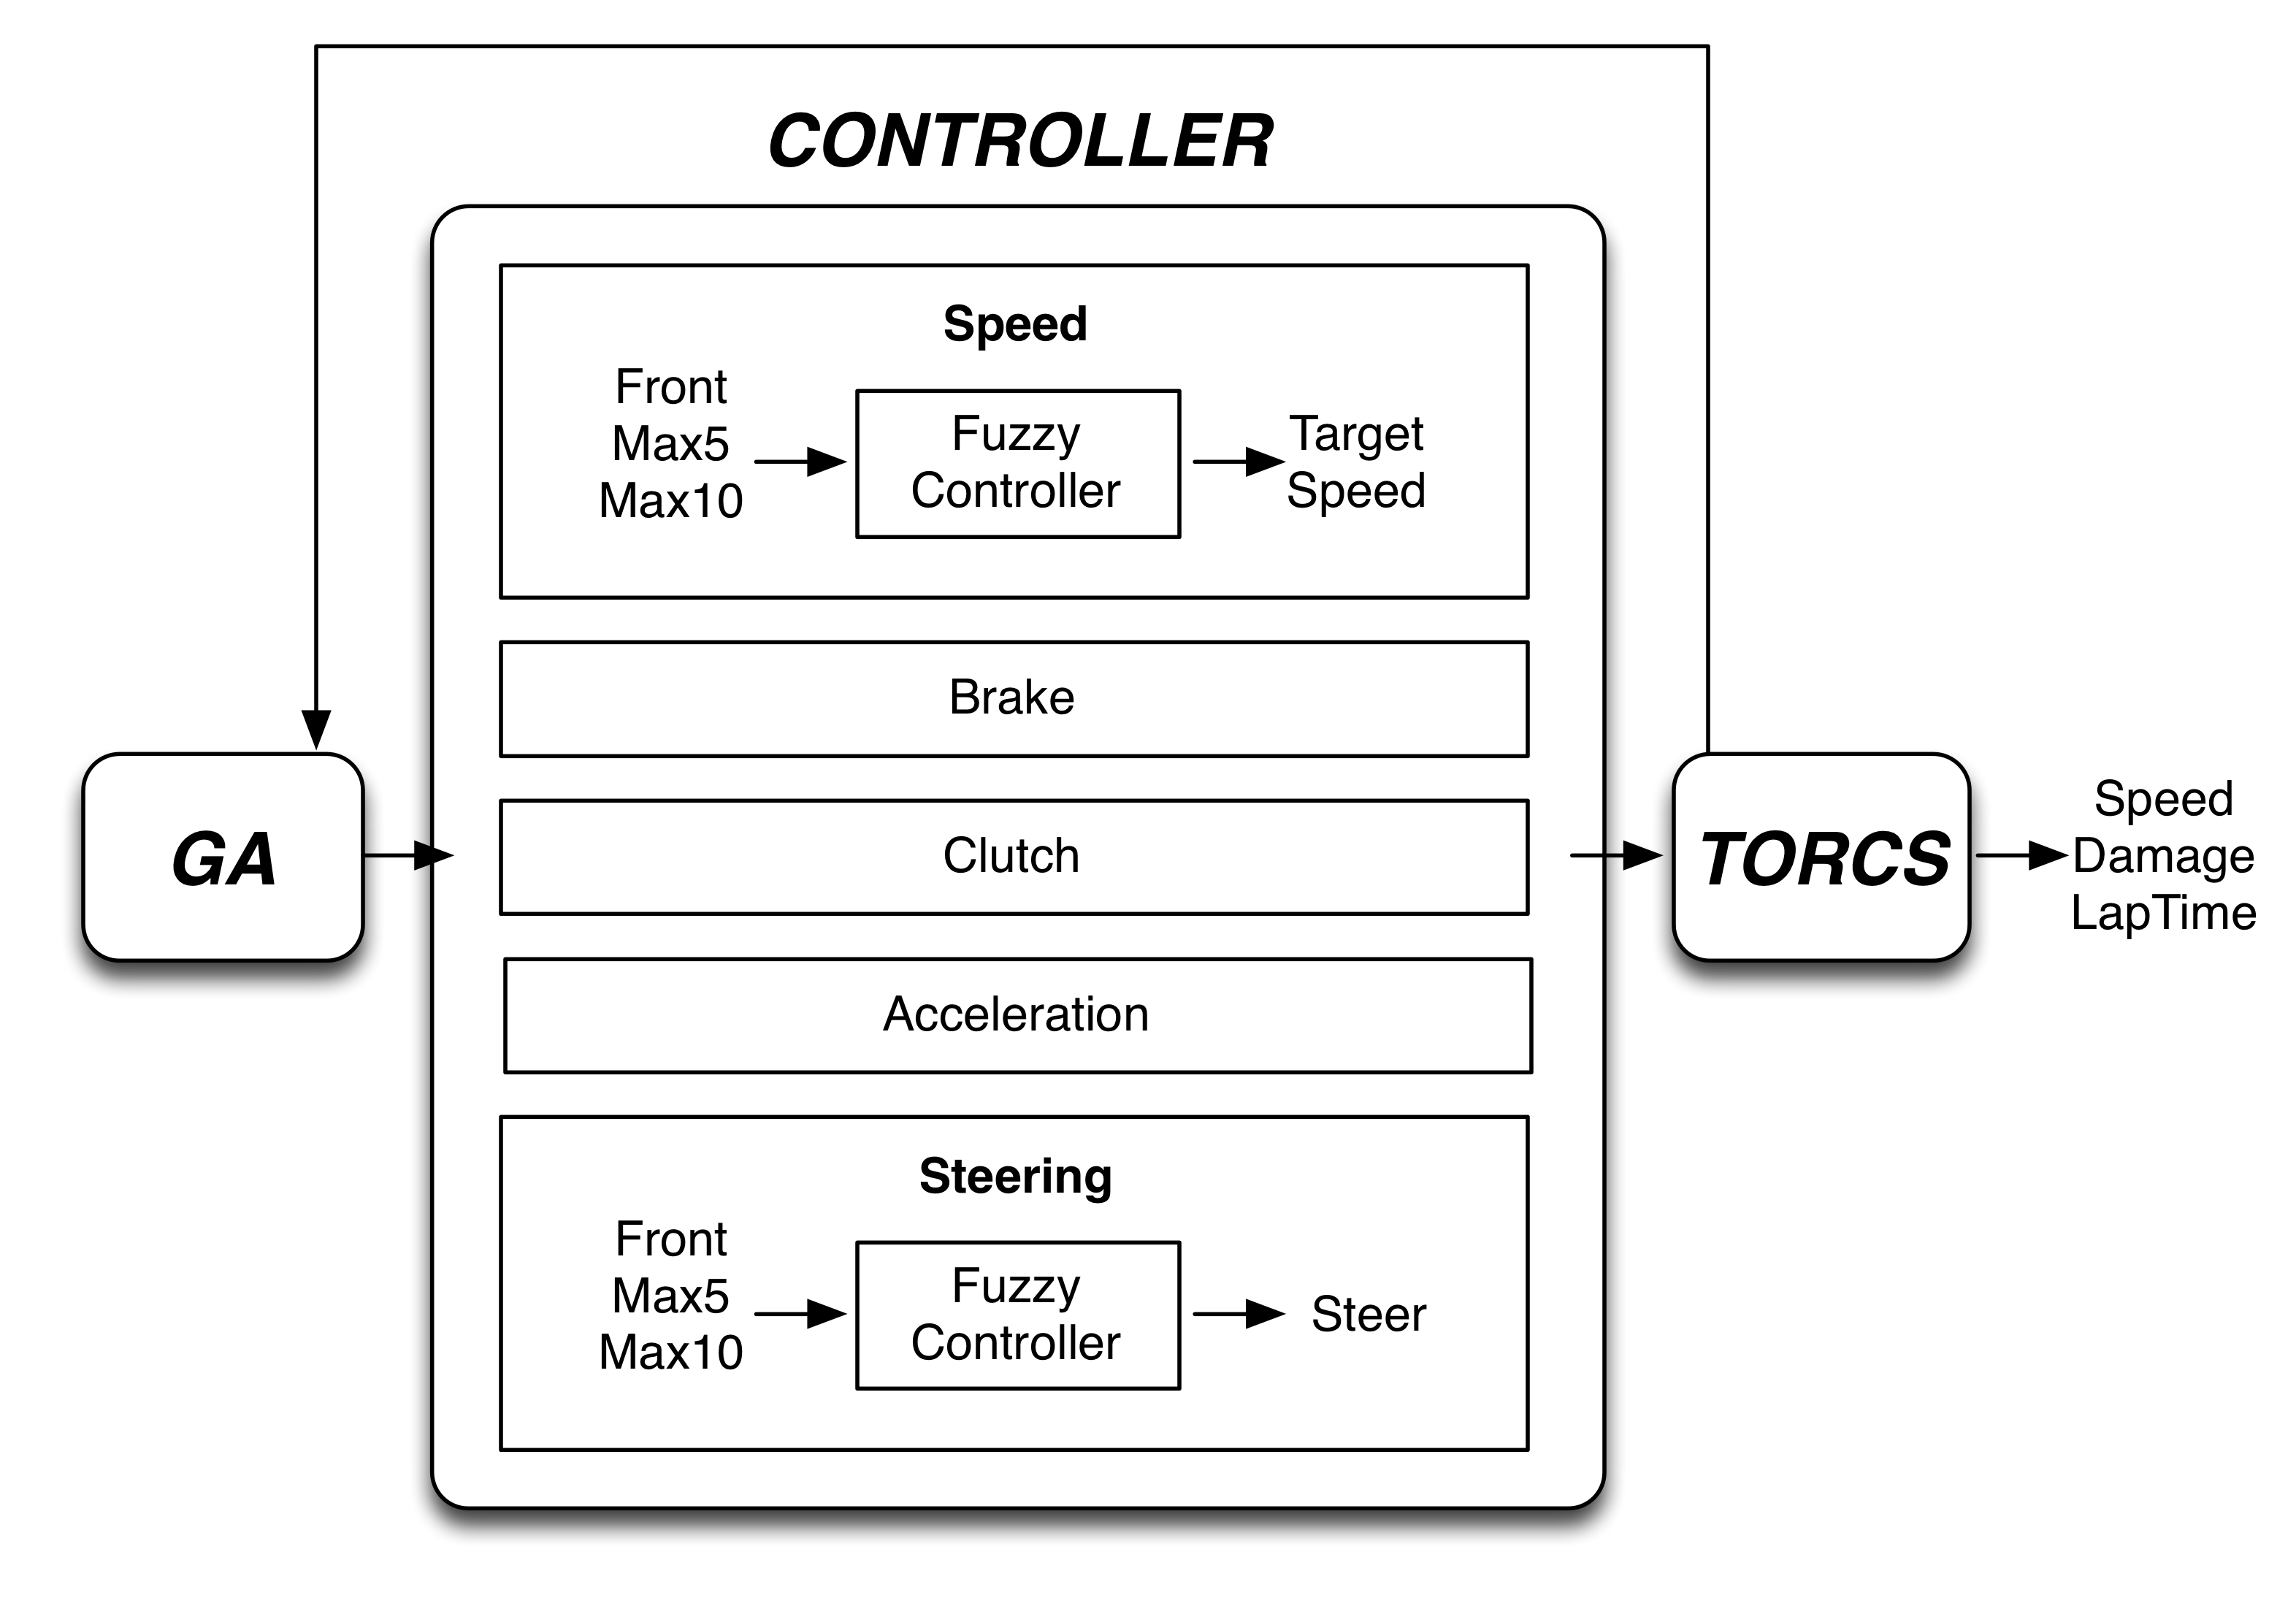
\includegraphics[width=10cm]{fig/flowchart}
	\end{center}
	\caption{Optimization of a fuzzy controller flowchart. The evaluation of an individual is performed by: putting the parameter values on the two sub-controllers, launching a race in TORCS with this configuration, obtaining the resulting values of Damage, Top Speed and mean Lap Time and using these values for the computation of the fitness of the individual.}
\end{figure}	

Indeed, the GA starts by creating the initial population with random values for the parameters in the defined range $[0,100]$. The fitness of each candidate solution is computed by injecting its gene values to the parameters of the membership functions of the two fuzzy sub-controllers. The defined autonomous controller is used to drive a car in a 20 laps race in E-Track5 circuit without opponents, and the results (Top speed, Damage and Mean Lap time) are used to compute the fitness value.


%***********************************************

\subsection{Genetic Algorithm settings}
%
As previously stated, the designed fuzzy controllers have trapezoidal membership functions given by Equation \ref{eq:trapmf}.
In such a controller, fuzzy rules are applied to linguistic terms. These terms, which qualify a linguistic variable, are defined through membership functions, which, in turn, depend on a set of parameters that `describes' their shape (and operation).

The parameters to be optimized are those of all the membership functions that constitute the fuzzy partition of the linguistic variable \cite{ThangG08}.

The input linguistic variables in our problem, \textit{Front, Max5} and \textit{Max10}, are represented by three trapezoidal membership functions (See Table \ref{tab:flouevar}).

A trapezoidal membership function in a finite universe of discourse \textit{[a, b]} can be defined by:

\begin{equation}
\mu_{A}(x)= \left \{
\begin{array}{ll}
\frac{x - x_{1}}{x_{2} - x_{1}},& x_{1} \leq x \leq x_{2}\\
1 , &x_{2} \leq x \leq x_{3}\\
\frac{x_{4} - x}{x_{4} - x_{3}},& x_{3} \leq x \leq x_{4}\\
0        ,& else\\	
\end{array}
\right.
\label{eq:trapmf}
\end{equation}
with:
\begin{equation}
x_{1} \leq x_{2} \leq x_{3} \leq x_{4}
\end{equation}
This MF function is defined by four parameters $x_{1}$, $x_{2}$, $x_{3}$ and $x_{4}$ taking their values in the interval \textit{[a, b]} (See Figure \ref{fig:trapeze}).																			
\begin{figure}[!ht] 
	\begin{center}
		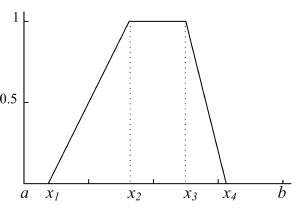
\includegraphics[scale=0.7]{fig/trapese}
		\caption {Trapezoidal MFs}
		\label{fig:trapeze}
	\end{center}
\end{figure}

More generally, a fuzzy partition with \textit{n} trapezoidal membership functions is defined by \textit{2n} variables (\textit{a =} $ x_{1}$,$x_{2} $,. .., $x_{2n} $ \textit {= b})(Equation \ref{eq:e1}). In this case, the representation is given by the figure \ref{fig:at}
\begin{figure}[!ht] 
	\begin{center}
		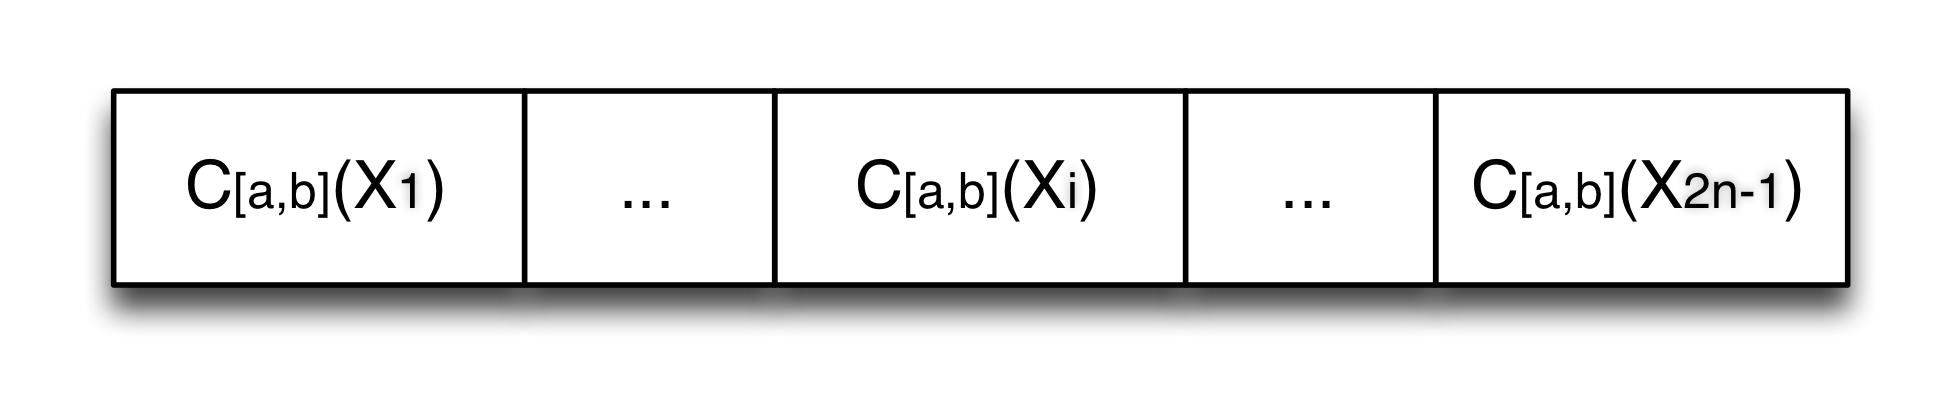
\includegraphics[scale=0.55]{fig/trapezoidal.png}
		\caption {Trapezoidal-shaped MFs coding}
		\label{fig:at}
	\end{center}
\end{figure}
with:
\begin{equation}
a = x_{1} \leq x_{2} \leq...\leq x_{2n-1} \leq x_{2n}=b 	
\end{equation}		

\begin{equation} 
\begin{tabular}{l}
$\mu_{A1}(x)=  \left \{
\begin{array}{ll}
1, &x_{1} \leq x \leq x_{2}\\
\frac{x_{3} - x}{x_{3} - x_{2}}, &x_{2} \leq x \leq x_{3}\\
0        , &x > x_{3}\\
\end{array} 
\right.$		\\ 	
$\mu_{Ai}(x)= \left \{
\begin{array}{ll} 
0, &x \leq x_{2i-2}\\
\frac{x - x_{2i-2}}{x_{2i-1} - x_{2i-2}}, &x_{2i-2} \leq x \leq x_{2i-1},n=2,...,i-1\\
1, & x_{2i-1} \leq x \leq x_{2i}\\
\frac{x_{2i+1} - x}{x_{2i+1} - x_{2i}},& x_{2i} \leq x \leq x_{2i+1}\\
0  , &x > x_{2i+1}\\
\end{array}  
\right.	$		\\
$\mu_{An}(x)= \left \{
\begin{array}{ll} 
0, &x \leq x_{2n-2}\\
\frac{x - x_{2n-2}}{x_{2n-1} - x_{2n-2}},& x_{2n-2} \leq x \leq x_{2n-1}\\
1 ,& x > x_{2n-1} 
\end{array} 
\right.$\\
\label{eq:e1}
\end{tabular}
\end{equation}
	
As we have just seen, a linguistic variable is represented by a number of parameters that depend both on the number and type of used membership functions  \cite{ThangG08}. Also the choice of coding to use for these different parameters depends both on the desired precision on the values and on their range of values.

When the number of parameters is reduced and their ranges of variations are well defined, a GA with a binary coding is largely sufficient to find their optimal values. On the other hand, if the number of parameters becomes important, and their variation interval is not well known, the real coding is the most appropriate \cite{elsayed13}. 
Since our work requires some precision and the variation interval of each parameter is not well known, we have considered a real coding implementation.

In that GA, every individual is a vector of 18 values/parameters, 6 per variable. Figure \ref {fig:cromosome} illustrates the structure of the chromosome.
\begin{figure}[!ht]	
	\begin{center}
		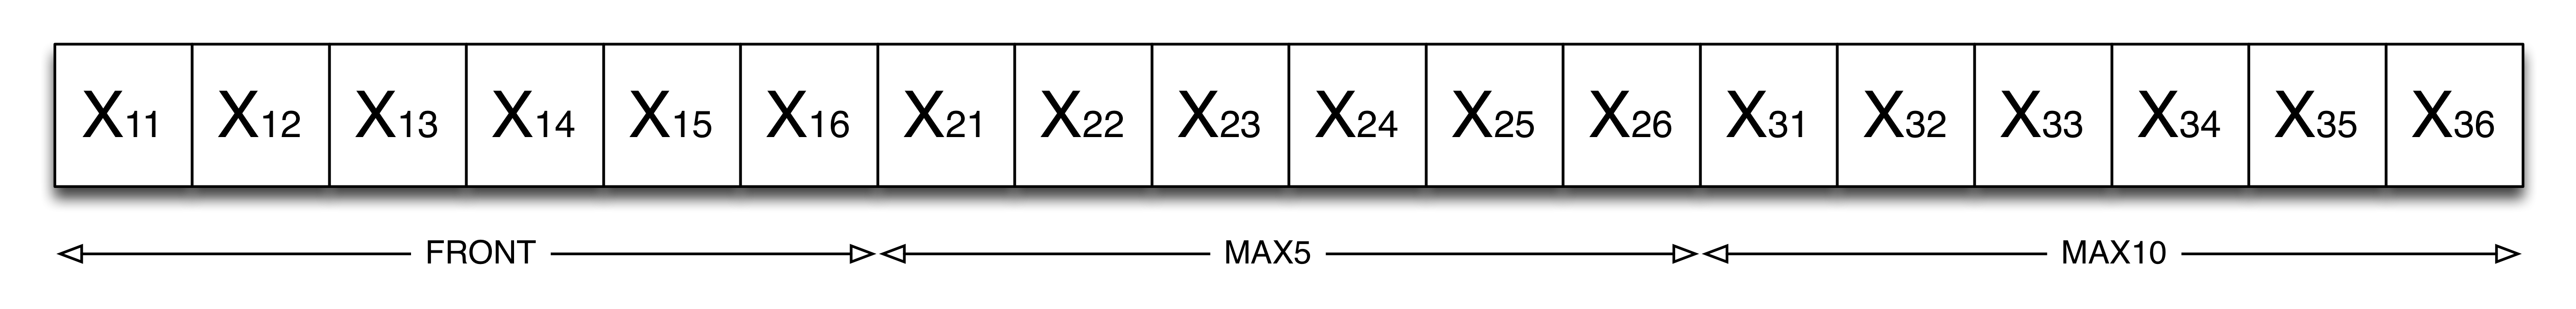
\includegraphics[width=12cm]{fig/chromosome2.png}
		\caption{Chromosome description}
		\label{fig:cromosome}	
	\end{center}	
\end{figure}

The initialization of the chromosomes (first population) is performed assigning random values inside a range of variation \cite{GAs_Goldberg89}, in order to start from feasible values \cite{evo17_blind}.
Tournament based selection has been used to elect chromosomes as parents for genetic operators, while simple arithmetic two point crossover \cite{crossGA2017} and non uniform mutation \cite{mutation1997} have been chosen, as two of the most contrasted methods in the literature.

%***********************************************

\subsection{Fitness definition}

The fitness function for optimizing the structure of a fuzzy controller is highly dependent on the application in which the controller is involved. It is therefore not possible to give a general formulation of this function able to adapt to all the peculiarities of a problem. However, we can specify some rules to choose the best evaluation function \cite{elsayed13}.

The fuzzy controller should aim to: 
\begin{itemize}
	\item  Minimize the damage of the car $damage$.
	\item  Minimize the mean of lap time $LapTime$.
	\item  Maximize the TopSpeed $MaxSpeed$.		
\end{itemize}

From these goals, we can derive two possible fitness functions:

\begin{description}
	\item[Fitness 1:]  
	\begin{equation} \label{fit1}
	\begin{array}{lllll}
	f_{1} =  Min & damage + &\alpha \cdot Min & LapTime 
	\end{array}
	\end{equation}
	\item[Fitness 2:] 
	\begin{equation} \label{fit2}
	\begin{array}{llllll}
	f_{2}= Min & damage + &\alpha \cdot Min & LapTime + & Min & \beta \cdot \frac{1}{TopSpeed}
	\end{array}
	\end{equation}	
\end{description}

Being $\alpha$ and $\beta$ two weighting parameters to prioritize the importance of the different objectives.
To evaluate the candidate controllers during the evolutionary process, we will make each of them compete in a 20 laps practice race in a medium difficulty circuit without rivals. We have omitted the presence of opponents in order to avoid including additional uncertainty sources to the optimization process.
% Antonio - Mohammed: which kind of race (practice or with rivals)? which kind of track? why this track?, which conditions (weather)?, which rivals?
%           This is very important to be mentioned and explained (why have these %           features been selected to correctly evaluate a controller). ;)
% Mohammed- Evaluation is in 20 laps to take the medium of lapstime 
% I  prefered not to include rivals because this  will increase the unknown parameters to take in account in optimization 
% Antonio - Ok, I have written that. ;)

Then, the obtained output values $damage$, $LapTime$ and $TopSpeed$ are collected to compute the corresponding fitness value. As a clarification, $LapTime$ is the average of the 20 laps time.

  		
%%%%%%%%%%%%%%%%%%%%%%%%%%%%  RESULTS  %%%%%%%%%%%%%%%%%%%%%%%%%%%%
	
\section{Results}  
\label{sec:results}
	
This section is dedicated to the performance evaluation of our
fuzzy-genetic controller, called \textit{FGC}. 

	
We will first need to choose whose tracks and cars are going to be used in the
experiment among the ones TORCS provides; in our case, we have selected the E-Track5 circuit as it is a
quite complex one, with multiple turns. \textit{car1-tbr1} has been
selected as the driving car \cite{evo17_blind}. According to previous
experiments, this is a fair choice due to its moderate
performance. This will lead our controller to be prepared to drive in the most usual conditions. 

We have evaluated the FGC with the two proposed fitness functions,
comparing them for racing performance. We have considered the following bots in the experiments, making 20 evolutionary runs for every one, with the configuration: Population size=20, Generations=50, Crossover rate=0.7, Mutation rate=0.3.
%shown in Table \ref{tab:GA_config}: 
%	
\begin{itemize}
\item \textbf{GFC1}: GA-Fuzzy controller with fitness 1 (Equation \ref{fit1}).
\item \textbf{GFC2}: GA-Fuzzy controller with fitness 2 (Equation \ref{fit2}).
\item \textbf{AD}: Fuzzy controller \cite{evo17_blind}.
\end{itemize}
%
%\begin{table}[!ht]	
%		\centering
%{\scriptsize
%		\caption{GA parameters}
%		\label{tab:GA_config}
%		\begin{tabular}{|p{3.6cm}|p{3cm}|}
%			\hline \textbf{Population size} & 20 \\
%			\hline \textbf{Generations} & 50   \\
%			\hline \textbf{Crossover rate$\textit{P}_{\textit{c}}$} &  0.7 \\
%			\hline \textbf{Mutation rate $\textit{P}_{\textit{m}}$} &  0.3   \\ 		
%			\hline          
%		\end{tabular}	
%}
%\end{table}

The coefficients $\alpha$ and $\beta$ are chosen to be $1$  and
$10*MaxSpeed$ respectively, where $MaxSpeed $ is the maximum value of
speed that \textit{car1-tbr1}  could take ($MaxSpeed=300$)
\cite{evo17_blind}, this choice is motivated by the fact to normalize
the Top speed values and make them in the same level as other fitness
terms. 
 The results of these runs are shown in Table \ref{tab:runsresults}.
 % Antonio - Comment the obtained values.
 % You can't publish a table with the individual runs, and even less
 % with a column for fitness. Fitness 1 and 2 are not
 % comparable. Publish just the best and average performance optained,
 % and also publish TopSpeed for Fitness 1 if it's logged - JJ
\begin{table}[ht]
	\centering
{\scriptsize
	\caption{ Results of 10 runs of GA with the two fitness
          functions. Please bear in mind that fitness follow different
        formula, and thus cannot be compared; LapTime and Damage
        should be the quantities used for comparison. }
	{
		\begin{tabular}{|c||c|c|c|c||c|c|c|c|}
			\hline
			 &\multicolumn{4}{c||}{Fitness 1}&\multicolumn{4}{c|}{Fitness 2}\\
			\cline{2-9}
			& Min fit. 1 & $LapTime$ & $Damage$ & $TopSpeed$& Min fit. 2& $LapTime$ & $Damage$ & $TopSpeed$\\
			\hline
			% 1 &46.42& 33.42& 13& 43.8005 & 30.98& 0& 234\\
			
			% 2 &31.09& 31.09& 0& 51.6614& 29.87& 11& 278\\
			
		 Best &\textbf{29.44}& 29.44& 0&231&\textbf{39.74} & 29.25& 0& 286\\
			
			% 4 &31.12& 31.12& 0& 60.5155& 31.64& 16& 233\\
			
			% 5 &39.63& 31.63&8&  41.7232 & 30.05& 0& 257\\
	            	
			% 6 &30.21& 30.21& 0&  41.8588 & 30.14& 0& 256\\
			
			% 7 &29.73& 29.73& 0& 40.3140 &29.12& 0& 268\\
			
			% 8 &37.29& 31.29&6& 40.8510 & 30.75& 0& 297\\
  			
			% 9 &34.07& 30.07& 4 & 40.8596 &29.99& 0& 276\\
			
			% 10&29.88& 29.88& 0& 40.0467&29.63& 0& 288\\
			\hline
			Mean &33.88 &30.79 &3.10&227.43&   44.14&  30.14 &   2.70&267.30\\ 
			St. Dev.&5.61&1.18&4.58&32.55&6.73&0.78 &5.81  & 22.03\\
			\hline
			
		\end{tabular}
	}\label{tab:runsresults}
}
\end{table}
% Mohammed - Best values and TopSpeed added
 From The Table, we can see that the $3^{rd}$ run has given the best fitness value for the two considered fitness functions and obtained the minimal Laptime and damage and for the second fitness , the higher TopSpeed in the track.  The fact that the GA  gave the minimum for two fitness functions  in the same run is due to the random initialization of the start population in a favorite region of the space search so the GA has found the optimal solution, as we used the same random start population to compare the two fitness functions. %Pablo: important! do not use so much parantheses, I have removed them. Check if the meaning of this paragraph is still correct
% Mohammed - ok, it's correct
 The worst values are obtained by $1^{st}$ Run for fitness 1 and $4^{th}$ run for the second fitness, thee bad values are produced by the damage when the car was in stuck or chocked with the track corner.
 The second fitness has given  higher Top Speed values  which minimize the Laptime and makes the controller operates at higher performances. Also, implying late breaking in turns which maximize the Top Speed.
 Wilcoxon rank sum non-parametric test \cite{garcia09} is used to reject or accept the null hypothesis of equality of medians of the values of the two fitness functions for the 10 runs. The obtained p-value was $p =  0.0017$ and the  test statistic is $stats = -3.1371$, this results lead to the rejection of null hypothesis with a threshold $\alpha=0.01$ which allows us to conclude that the two samples sets are different.
 
 % Mohammed - Runs were deleted by JJ ,could we  cite runs that are not in the Table???
% Antonio - Yes, I think we can now say the did 20 runs instead of 10. ;)

The best solution obtained with each fitness function from these runs have been considered to be tested. %Pablo: to be tested where?
We represented the resulted membership functions of these two optimal individuals considering the different fitness functions in Figures \ref{fig:mffront}, \ref{fig:mfmax5} and \ref{fig:MFMAX10}.

\begin{figure}%
	\centering
	\subfigure[with Fitness 1]{%
		\label{fig:front1}%
		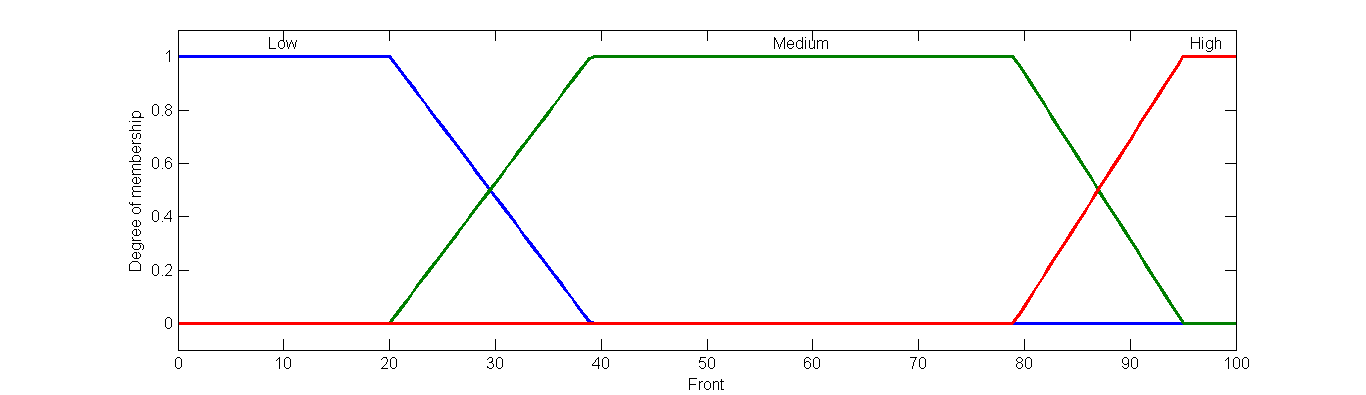
\includegraphics[width=0.6\textwidth,height=3cm]{fig/MFFRONT}}%
	\subfigure[with Fitness 2]{%
		\label{fig:front2}%
		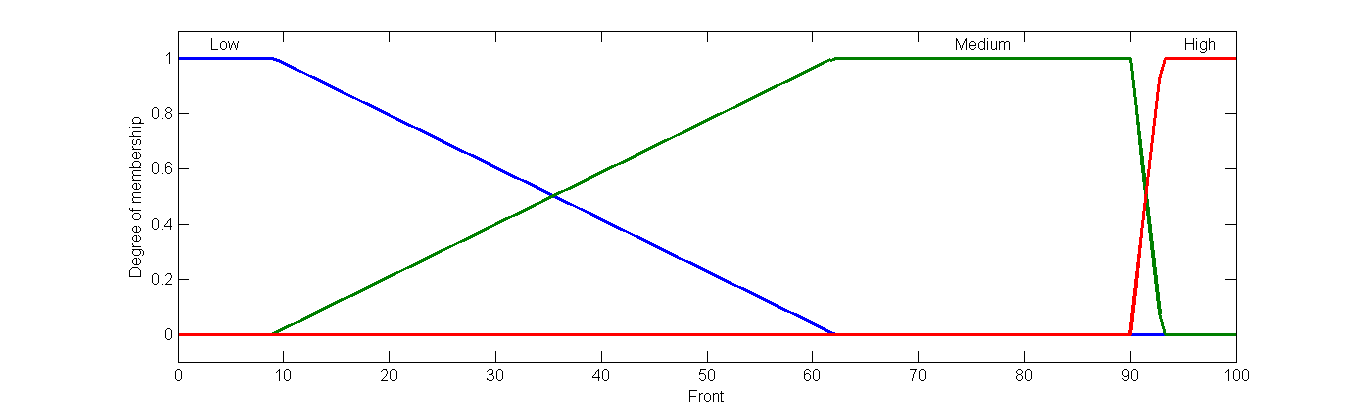
\includegraphics[width=0.6\textwidth,height=3cm]{fig/MFFRONT2}}%
	\caption{Front input MFs with GA}
	\label{fig:mffront}
\end{figure}
%
\begin{figure}%
	\centering
	\subfigure[with Fitness 1]{%
		\label{fig:fmax51}%
		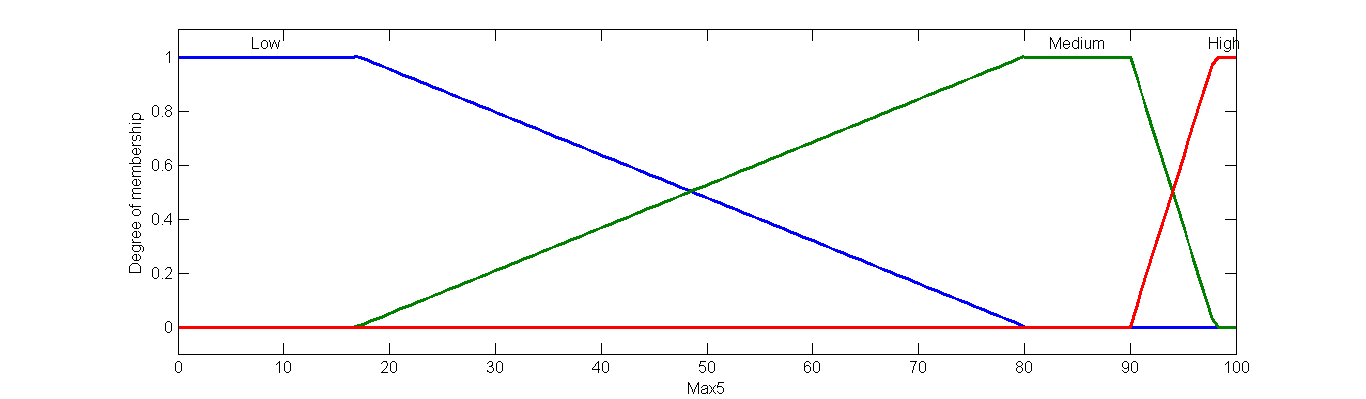
\includegraphics[width=0.6\textwidth,height=3cm]{fig/MFFMAX5}}%
	\subfigure[with Fitness 2]{%
		\label{fig:fmax52}%
		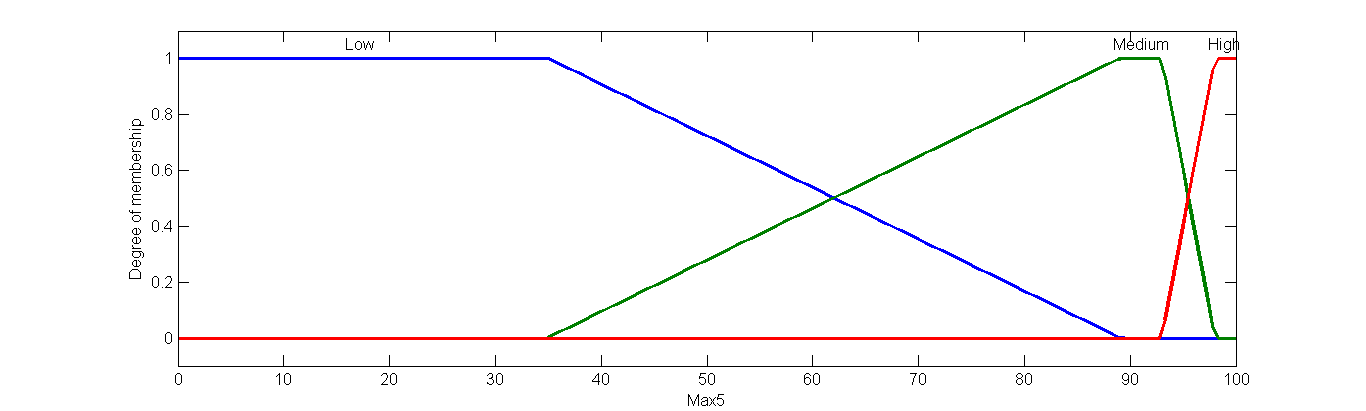
\includegraphics[width=0.6\textwidth,height=3cm]{fig/MFFMAX52}}%
	\caption{Max5 input MFs with GA}
	\label{fig:mfmax5}%
\end{figure}
%
\begin{figure}%
	\centering
	\subfigure[with Fitness 1]{%
		\label{fig:MFMAX101}%
		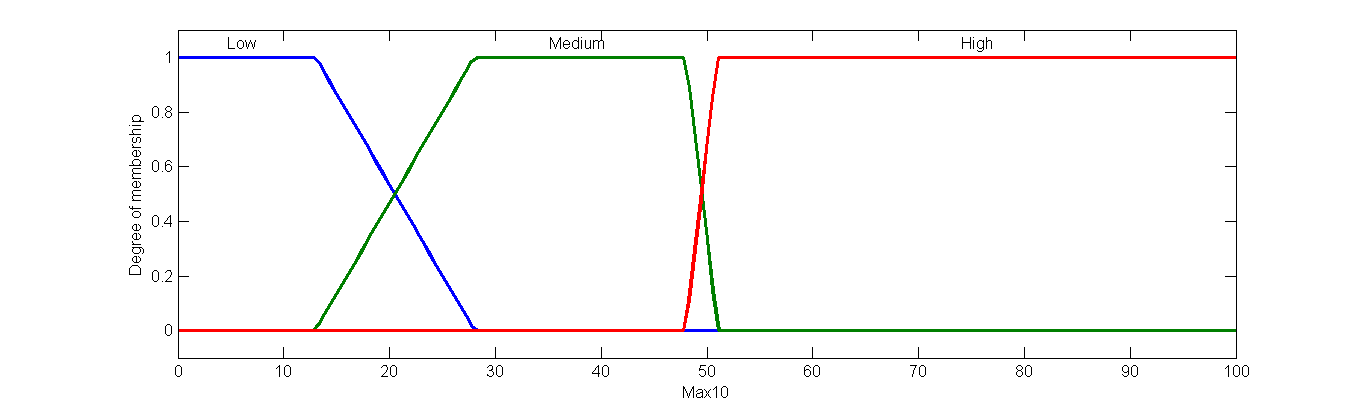
\includegraphics[width=0.6\textwidth,height=3cm]{fig/MFMAX10}}%
	\subfigure[with Fitness 2]{%
		\label{fig:MFMAX102}%
		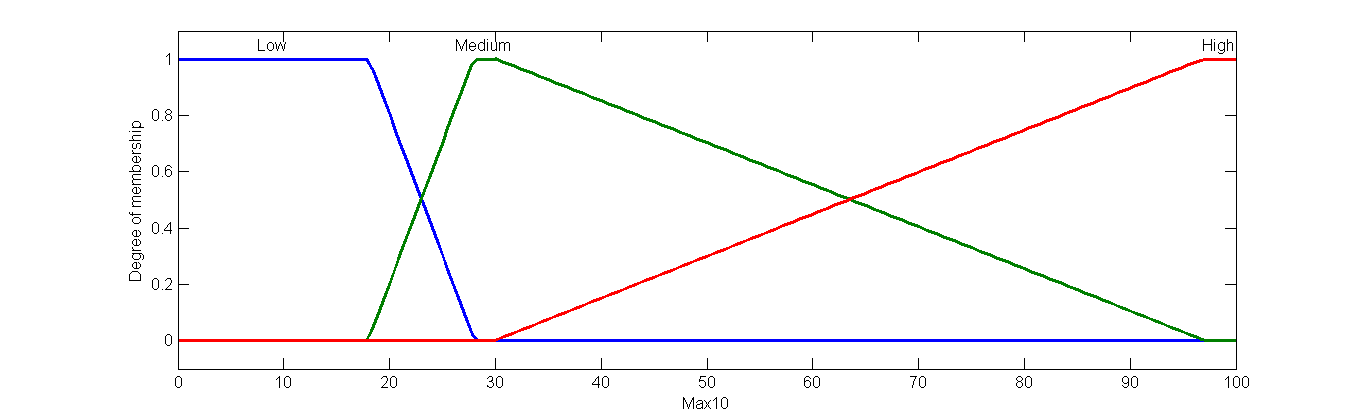
\includegraphics[width=0.6\textwidth,height=3cm]{fig/MFMAX102}}%
	\caption{Max10 input MFs with GA}
		\label{fig:MFMAX10}%
\end{figure}

The shapes of the obtained memberships are completely different from
those obtained by Trial/Error in the previous work \cite{evo17_blind}
where the Medium linguistic variable of the new functions has bigger
range. This makes the controller very sensitive to the middle
distances of the inputs, like for a real driver who considers most of
the cases the car distance from the borders in that range. 
The other remark from the obtained  membership functions is the
dimension of the common range between the LOW and MEDIUM, which
provide a higher diversity in the output values. 


%%%%%%%%%%%%%%%%%%%%%%%%%%%%%%%%%%%%%%%%%%%%%%%%%%%%%

The two best genetic based fuzzy controllers obtained in the previous
experiments, one per fitness function and thus named $GFC1$ and
$GFC2$, are going to be tested
in a practice race together with the $AD$ fuzzy controller which we
have considered as a base line. They will run
each one for 20 laps in E-Track5 circuit, which was the one used during the
evolution; then, they will be tested also in a practice race in
E-Road, a track they had not encountered previously. The obtained results are presented
in Table \ref{resultat20}. 

\begin{table}[!ht]
	\centering
	{\scriptsize
		\caption{Results of the three controllers in a 20 laps practice race}
		\label{resultat20}
		\begin{tabular}{|p{3cm}|c|c|c|}
			\hline
			\multicolumn{4}{|c|}{\textbf{E-Track 5}}  \\
			\hline \textbf{Results} & & \textbf{GFC1} & \textbf{GFC2}  \\
			\hline Best Lap Time         & & 30:01 & 29:21 \\
			\hline Top Speed          &  & 224 & 234\\
			\hline Min Speed          &  & 151 & 186 \\
			\hline Damage          & & 0 & 0\\
			\hline 
			\hline
			\multicolumn{4}{|c|}{\textbf{CG Track2}}  \\ 
			\hline \textbf{Results} & & \textbf{GFC1} & \textbf{GFC2}  \\
			\hline Best Lap Time         &     &   01:04:96     & 01:02:32  \\
			\hline Top Speed& &220  &  238 \\
			\hline Min Speed          &      & 33             & 40  \\
			\hline Damage          &   0         & 0              & 0  \\
			\hline 
		\end{tabular}
	}
\end{table}
% Antonio - Mohammed, please check the values of the first track (E-Track 5) as the best lap and the last lap times are always the same (for the 3 controllers).
%Mohammed- The second controller  obtained the best lap in the last one, for the other , I corrected it
% Antonio - Great. :)
% They are still too similar. Since there are 20 laps, you should
% perform a statistical test of difference between GFC1 and 2. - JJ
% Mohammed - it could be done but it needs more then 30 runs to apply
% nonparametric tests ( Wilcoxon or others, normality condition is not
% verified for the Data of the two controllers)
% You don't need normality to apply Wilcoxon. You could also show a
% chart to highlight differences - JJ
From the table, we can see that the fuzzy controllers optimized by the
GA have given the best results, minimizing the global race time and
damages ($0$ in the two GA-based fuzzy controllers), while the AD
controller has finished the practice race with many damages.
% But the difference is a few seconds. Still the statistical test
% should be mentioned - JJ
Testing the controllers in this E-Road, which is quite long and
difficult as it can be seen by the time it takes a single lap, has proved their value in the adaptation to other
tracks different from the one used for `training', that is, the
optimization of the fuzzy controllers.
% I have eliminated parentheses here. Please avoid them in formal
% writing - JJ

The GFC2 controller has run with a higher speed (considering overall Top
Speed and Min Speed) than GFC1 in the two tracks. This is a positive
consequence of the inclusion of the $TopSpeed$ variable in the fitness
computation so the GA based fuzzy controller has optimized the speed
of the car due to early braking and detection of turns and their
curving angles. This ability  of the GA-fuzzy controller collaborates
to minimize the overall race time and thus the final ranking.
% Antonio - add more comments on the results
% Mohammed- done
According to these results, GFC2 seems to be the best controller.
% Not sure about this. Difference is very small. More test should be
% done on an E-Road, maybe 15 (always minimum in statistics). They
% seem too similar and are probably not statistically different - JJ
% We'll leave that to the next paper, but we still have to mention
% that there is a statistical difference.

%%%%%%%%%%%%%%%%%%%%%%%%%%%%%%%%%%%%%%%%%%%%%%%%%%%%%
% You can't simply drop the reader into the next experiment. It has to
% be "narrated", linked to the previous paragraphs and justified. For
% instance - jj
Comparing average lap time gives us an overall idea of which
controller performs the best; however, at the end of the day in a
racing game the race has to be won. That is why we have tested every
fuzzy separately from the others in a real race against five standard controllers from each team integrated with TORCS. Tables \ref{tab:gfc1real} and \ref{tab:gfc2real}   illustrate their performance in two 5 laps real races.  % Which track? - JJ
\begin{table}[!ht]
	\centering
	{\scriptsize
		\caption{Results of GFC1 in two real races (5 laps)}
		% Explain the "Race time" row - JJ
		\label{tab:gfc1real}
		\begin{tabular}{|p{2 cm}|p{1.5 cm}|p{1.5 cm}|p{1.5 cm}|p{1.5 cm}|p{1.5 cm}|p{1.5 cm}|}
			\hline \textbf{E-TRACK5} &   \textbf{GFC1} & \textbf{berwin 10} & \textbf{bt 3} &\textbf{damned 2} & \textbf{inferno 5} & \textbf{tita 10}  \\
			\hline \textbf{Ranking} & 3/6&4/6&1/6&5/6&2/6&6/6\\			
			\hline \textbf{Race Time}	& 02:29:32\newline+24:11&02:29:32\newline +1 lap &02:29:32&02:29:32\newline +1 lap &02:29:32\newline+13:67&02:29:32\newline+1 lap\\	
			\hline \textbf{Best Lap}&33:79& 35:39&28:09&36:73&31:49&34:12\\	
			\hline \textbf{Max Speed}& 199&206&233&198&229&219\\	
			\hline \textbf{Damages}& 0&0&0&599&7&566 \\	
			\hline 
		\end{tabular}
		
		\begin{tabular}{|p{2 cm}|p{1.5 cm}|p{1.5 cm}|p{1.5 cm}|p{1.5 cm}|p{1.5 cm}|p{1.5 cm}|}
			\hline \textbf{CG Track2} & \textbf{GFC1}&\textbf{berwin 10} & \textbf{bt 3} &\textbf{damned 2} & \textbf{inferno 5} & \textbf{tita 10}  \\
			\hline \textbf{Ranking} & 3/6&4/6&1/6&6/6&5/6&2/6\\			
			\hline \textbf{Race Time}	&  05:10:66\newline +25:43&  05:10:66\newline+55:65& 05:10:66& 05:10:66\newline+1 lap& 05:10:66\newline+38:44& 05:10:66\newline+19:82\\	
			\hline \textbf{Best Time}& 1:03:65 &1:04:21&1:00:57&1:04:26&1:03:19&1:03:98\\	
			\hline \textbf{Max Speed}& 233&236&288&200&238&229\\
			\hline \textbf{Damage}& 112& 376 & 433&988&541&890\\	
			\hline 
		\end{tabular}
	}
\end{table}


\begin{table}[!ht]
	\centering
{\scriptsize
	\caption{Results of GFC2 in two real races (5 laps)}
	\label{tab:gfc2real}
	\begin{tabular}{|p{2 cm}|p{1.5 cm}|p{1.5 cm}|p{1.5 cm}|p{1.5 cm}|p{1.5 cm}|p{1.5 cm}|}
		\hline \textbf{E-TRACK5} & \textbf{GFC2}&\textbf{berwin 10} & \textbf{bt 3} &\textbf{damned 2} & \textbf{inferno 5} & \textbf{tita 10}  \\
		\hline \textbf{Ranking} & 2/6&4/6&1/6&6/6&3/6&5/6\\			
		\hline \textbf{Race Time}	& 02:30:83\newline +03:99&  02:30:83\newline+1 lap&02:30:83&02:30:83\newline+1 lap&02:30:83\newline+08:35&02:30:83\newline+1 lap\\	
		\hline \textbf{Best Time}& 29:82 &36:38&28:35&37:04&30:53&36:00\\	
		\hline \textbf{Max Speed}& 214&202&230&188&226&204\\	
		\hline \textbf{Damage}& 0& 0 & 343&1230&0&668\\	
		\hline 
	\end{tabular}

	\begin{tabular}{|p{2 cm}|p{1.5 cm}|p{1.5 cm}|p{1.5 cm}|p{1.5 cm}|p{1.5 cm}|p{1.5 cm}|}
		\hline \textbf{E-ROAD} & \textbf{GFC2}&\textbf{berwin 10} & \textbf{bt 3} &\textbf{damned 2} & \textbf{inferno 5} & \textbf{tita 10}  \\
		\hline \textbf{Ranking} & 3/6&4/6&1/6&6/6&2/6&5/6\\			
		\hline \textbf{Race Time}	& 05:38:23\newline +17:72&  05:38:23\newline+1 lap&05:38:23&05:38:23\newline+1 lap&05:38:23\newline+10:73&05:38:23\newline+1 lap\\	
		\hline \textbf{Best Time}& 1:17:34 &1:16:29&1:14:97&1:20:80&1:13:98&1:15:29\\	
		\hline \textbf{Max Speed}& 221&206&228&178&228&206\\
		\hline \textbf{Damage}& 120& 356 & 753&2750&130&894\\	
		\hline 
	\end{tabular}
}
\end{table}

First of all, as it can be seen, the original controller AD has had a poor performance, getting the last position in both races.
Whereas both $GFC1$ and $GFC2$ controllers showed to be more competitive. 
GFC2 has got an excellent second position in the track used during optimization (E-Track), and it has also got a remarkable third rank in the unknown track (E-Road). 
Both controllers have dealt very well for not being damaged, which even the winner, {\tt bt 3}, could not avoid. 

These results are a confirmation of the good optimization done by the GA and mainly when the Top Speed was considered in the fitness. 
The obtained results in real race with opponents from tough teams from TORCS are encouraging even the optimization process was in practice races.
This good adaptation of the proposed controller in races with rivals is due to the fact the modular fuzzy controller takes into consideration the presence of rivals in the track \cite{evo17_blind}. 
The enhancement of that driver by the optimal values of the membership function values, allows it to detect and overtake the opponents with no damage or stuck.
 
%%%%%%%%%%%%%%%%%%%%%%%%%%%%  CONCLUSIONS  %%%%%%%%%%%%%%%%%%%%%%%%%%%%
\section{Conclusions and Future Work} 
\label{sec:conclusions}

In this work, we have presented an improved Genetic Algorithm implementation that 
optimizes and improves autonomous  driving using fuzzy systems for TORCS simulator
\cite{evo17_blind}, which combines two sub-controllers, one to
calculate the target speed and the other for the direction, that is, for driving the steering wheel. . 

After initial tests, that showed the promise of this approach, and
where we experimented with two different fitness functions, one
considering the average lap time and the car damage and another adding
the top speed reached, we have fine-tuned some algorithm parameters to
obtain better results. As in the initial tests, the fuzzy-genetic
controllers obtained were compared with the original AD controller
whose parameters were determined empirically. The comparison was made
first without opponents and then including several cars from the TORCS
teams in realistic races. 

The obtained results are very promising since the optimized
controllers overcome the original in the practice races, and also they
were ranked among the first ones in the evaluation races, with the
minimum of damage.

% Say something about how much better this one was compared with the first.


% We have to revise this. 
Nevertheless, these results can be improved by extending the
evaluation of population controllers in the Genetic algorithm to other
tracks and not just one, to allow the elected controller to practice
effectively in multiple tracks and in real-life situations. 
Moreover, we could also try to generate, optimize and tune automatically the rule base of the fuzzy controller by means of a Genetic Programming algorithm. %Pablo: also mention the possibility of Multi-Objective EAs.


\section*{Acknowledgments}

This work has been supported in part by: Ministerio espa\~{n}ol de
Econom\'{\i}a y Competitividad under project TIN2014-56494-C4-3-P
(UGR-EPHEMECH).


	\bibliographystyle{splncs03}
	\bibliography{fuzzy_torcs}

\end{document}
